% Options for packages loaded elsewhere
\PassOptionsToPackage{unicode}{hyperref}
\PassOptionsToPackage{hyphens}{url}
%
\documentclass[
]{article}
\title{Homework 3 - FE 570}
\author{Siddharth Iyer}
\date{3/30/2022}

\usepackage{amsmath,amssymb}
\usepackage{lmodern}
\usepackage{iftex}
\ifPDFTeX
  \usepackage[T1]{fontenc}
  \usepackage[utf8]{inputenc}
  \usepackage{textcomp} % provide euro and other symbols
\else % if luatex or xetex
  \usepackage{unicode-math}
  \defaultfontfeatures{Scale=MatchLowercase}
  \defaultfontfeatures[\rmfamily]{Ligatures=TeX,Scale=1}
\fi
% Use upquote if available, for straight quotes in verbatim environments
\IfFileExists{upquote.sty}{\usepackage{upquote}}{}
\IfFileExists{microtype.sty}{% use microtype if available
  \usepackage[]{microtype}
  \UseMicrotypeSet[protrusion]{basicmath} % disable protrusion for tt fonts
}{}
\makeatletter
\@ifundefined{KOMAClassName}{% if non-KOMA class
  \IfFileExists{parskip.sty}{%
    \usepackage{parskip}
  }{% else
    \setlength{\parindent}{0pt}
    \setlength{\parskip}{6pt plus 2pt minus 1pt}}
}{% if KOMA class
  \KOMAoptions{parskip=half}}
\makeatother
\usepackage{xcolor}
\IfFileExists{xurl.sty}{\usepackage{xurl}}{} % add URL line breaks if available
\IfFileExists{bookmark.sty}{\usepackage{bookmark}}{\usepackage{hyperref}}
\hypersetup{
  pdftitle={Homework 3 - FE 570},
  pdfauthor={Siddharth Iyer},
  hidelinks,
  pdfcreator={LaTeX via pandoc}}
\urlstyle{same} % disable monospaced font for URLs
\usepackage[margin=1in]{geometry}
\usepackage{color}
\usepackage{fancyvrb}
\newcommand{\VerbBar}{|}
\newcommand{\VERB}{\Verb[commandchars=\\\{\}]}
\DefineVerbatimEnvironment{Highlighting}{Verbatim}{commandchars=\\\{\}}
% Add ',fontsize=\small' for more characters per line
\usepackage{framed}
\definecolor{shadecolor}{RGB}{248,248,248}
\newenvironment{Shaded}{\begin{snugshade}}{\end{snugshade}}
\newcommand{\AlertTok}[1]{\textcolor[rgb]{0.94,0.16,0.16}{#1}}
\newcommand{\AnnotationTok}[1]{\textcolor[rgb]{0.56,0.35,0.01}{\textbf{\textit{#1}}}}
\newcommand{\AttributeTok}[1]{\textcolor[rgb]{0.77,0.63,0.00}{#1}}
\newcommand{\BaseNTok}[1]{\textcolor[rgb]{0.00,0.00,0.81}{#1}}
\newcommand{\BuiltInTok}[1]{#1}
\newcommand{\CharTok}[1]{\textcolor[rgb]{0.31,0.60,0.02}{#1}}
\newcommand{\CommentTok}[1]{\textcolor[rgb]{0.56,0.35,0.01}{\textit{#1}}}
\newcommand{\CommentVarTok}[1]{\textcolor[rgb]{0.56,0.35,0.01}{\textbf{\textit{#1}}}}
\newcommand{\ConstantTok}[1]{\textcolor[rgb]{0.00,0.00,0.00}{#1}}
\newcommand{\ControlFlowTok}[1]{\textcolor[rgb]{0.13,0.29,0.53}{\textbf{#1}}}
\newcommand{\DataTypeTok}[1]{\textcolor[rgb]{0.13,0.29,0.53}{#1}}
\newcommand{\DecValTok}[1]{\textcolor[rgb]{0.00,0.00,0.81}{#1}}
\newcommand{\DocumentationTok}[1]{\textcolor[rgb]{0.56,0.35,0.01}{\textbf{\textit{#1}}}}
\newcommand{\ErrorTok}[1]{\textcolor[rgb]{0.64,0.00,0.00}{\textbf{#1}}}
\newcommand{\ExtensionTok}[1]{#1}
\newcommand{\FloatTok}[1]{\textcolor[rgb]{0.00,0.00,0.81}{#1}}
\newcommand{\FunctionTok}[1]{\textcolor[rgb]{0.00,0.00,0.00}{#1}}
\newcommand{\ImportTok}[1]{#1}
\newcommand{\InformationTok}[1]{\textcolor[rgb]{0.56,0.35,0.01}{\textbf{\textit{#1}}}}
\newcommand{\KeywordTok}[1]{\textcolor[rgb]{0.13,0.29,0.53}{\textbf{#1}}}
\newcommand{\NormalTok}[1]{#1}
\newcommand{\OperatorTok}[1]{\textcolor[rgb]{0.81,0.36,0.00}{\textbf{#1}}}
\newcommand{\OtherTok}[1]{\textcolor[rgb]{0.56,0.35,0.01}{#1}}
\newcommand{\PreprocessorTok}[1]{\textcolor[rgb]{0.56,0.35,0.01}{\textit{#1}}}
\newcommand{\RegionMarkerTok}[1]{#1}
\newcommand{\SpecialCharTok}[1]{\textcolor[rgb]{0.00,0.00,0.00}{#1}}
\newcommand{\SpecialStringTok}[1]{\textcolor[rgb]{0.31,0.60,0.02}{#1}}
\newcommand{\StringTok}[1]{\textcolor[rgb]{0.31,0.60,0.02}{#1}}
\newcommand{\VariableTok}[1]{\textcolor[rgb]{0.00,0.00,0.00}{#1}}
\newcommand{\VerbatimStringTok}[1]{\textcolor[rgb]{0.31,0.60,0.02}{#1}}
\newcommand{\WarningTok}[1]{\textcolor[rgb]{0.56,0.35,0.01}{\textbf{\textit{#1}}}}
\usepackage{graphicx}
\makeatletter
\def\maxwidth{\ifdim\Gin@nat@width>\linewidth\linewidth\else\Gin@nat@width\fi}
\def\maxheight{\ifdim\Gin@nat@height>\textheight\textheight\else\Gin@nat@height\fi}
\makeatother
% Scale images if necessary, so that they will not overflow the page
% margins by default, and it is still possible to overwrite the defaults
% using explicit options in \includegraphics[width, height, ...]{}
\setkeys{Gin}{width=\maxwidth,height=\maxheight,keepaspectratio}
% Set default figure placement to htbp
\makeatletter
\def\fps@figure{htbp}
\makeatother
\setlength{\emergencystretch}{3em} % prevent overfull lines
\providecommand{\tightlist}{%
  \setlength{\itemsep}{0pt}\setlength{\parskip}{0pt}}
\setcounter{secnumdepth}{-\maxdimen} % remove section numbering
\ifLuaTeX
  \usepackage{selnolig}  % disable illegal ligatures
\fi

\begin{document}
\maketitle

Packages

\begin{Shaded}
\begin{Highlighting}[]
\FunctionTok{library}\NormalTok{(xts)}
\FunctionTok{library}\NormalTok{(highfrequency)}
\end{Highlighting}
\end{Shaded}

Load Dataset

\begin{Shaded}
\begin{Highlighting}[]
\CommentTok{\# load the TAQ dataset}
\FunctionTok{Sys.setenv}\NormalTok{(}\AttributeTok{TZ =} \StringTok{"GMT"}\NormalTok{) }\CommentTok{\# work in East Coast Time Zone}
\FunctionTok{options}\NormalTok{(}\AttributeTok{digits.secs=}\DecValTok{3}\NormalTok{)}
\FunctionTok{load}\NormalTok{(}\StringTok{"sampleTQdata.RData"}\NormalTok{)}
\end{Highlighting}
\end{Shaded}

Problem 3.1.1: Calibrate Roll Model

\begin{Shaded}
\begin{Highlighting}[]
\CommentTok{\# Calibrate the Roll model on the tqdata}
\NormalTok{pr }\OtherTok{\textless{}{-}} \FunctionTok{as.numeric}\NormalTok{(tqdata}\SpecialCharTok{$}\NormalTok{PRICE)}
\NormalTok{dpr }\OtherTok{\textless{}{-}} \FunctionTok{diff}\NormalTok{(pr)  }\CommentTok{\# Delta price}
\NormalTok{acpr }\OtherTok{\textless{}{-}} \FunctionTok{acf}\NormalTok{(dpr, }\AttributeTok{lag.max=}\DecValTok{20}\NormalTok{, }\AttributeTok{type=}\StringTok{"correlation"}\NormalTok{, }
            \AttributeTok{plot=}\ConstantTok{TRUE}\NormalTok{, }\AttributeTok{main=}\StringTok{"Autocorrelation"}\NormalTok{)}
\end{Highlighting}
\end{Shaded}

\includegraphics{hw3---siddharth-iyer_files/figure-latex/unnamed-chunk-3-1.pdf}

\begin{Shaded}
\begin{Highlighting}[]
\CommentTok{\# acf: both autocorrelation and autocovariance}

\FunctionTok{plot}\NormalTok{(acpr, }\AttributeTok{col=}\StringTok{"red"}\NormalTok{, }\AttributeTok{lag.max=}\DecValTok{20}\NormalTok{, }
     \AttributeTok{main=}\StringTok{"Autocorrelation of price changes"}\NormalTok{)}
\end{Highlighting}
\end{Shaded}

\includegraphics{hw3---siddharth-iyer_files/figure-latex/unnamed-chunk-3-2.pdf}

\begin{Shaded}
\begin{Highlighting}[]
\CommentTok{\# Roll estimate of bid{-}ask spread}

\NormalTok{covpr }\OtherTok{\textless{}{-}} \FunctionTok{acf}\NormalTok{(dpr, }\AttributeTok{lag.max=}\DecValTok{20}\NormalTok{, }\AttributeTok{type=}\StringTok{"covariance"}\NormalTok{, }\AttributeTok{plot=}\ConstantTok{FALSE}\NormalTok{)}

\NormalTok{gamma0 }\OtherTok{\textless{}{-}} \FunctionTok{sd}\NormalTok{(dpr)}\SpecialCharTok{\^{}}\DecValTok{2}
\CommentTok{\#print(gamma0)}

\NormalTok{gamma0alt }\OtherTok{\textless{}{-}}\NormalTok{ covpr}\SpecialCharTok{$}\NormalTok{acf[}\DecValTok{1}\NormalTok{]}
\CommentTok{\#print(gamma0alt)}

\NormalTok{gamma1 }\OtherTok{\textless{}{-}}\NormalTok{ covpr}\SpecialCharTok{$}\NormalTok{acf[}\DecValTok{2}\NormalTok{]}
\CommentTok{\#print(gamma1)}

\NormalTok{cparam}\FloatTok{.1} \OtherTok{\textless{}{-}} \FunctionTok{sqrt}\NormalTok{(}\SpecialCharTok{{-}}\NormalTok{covpr}\SpecialCharTok{$}\NormalTok{acf[}\DecValTok{2}\NormalTok{])}
\FunctionTok{cat}\NormalTok{(}\StringTok{"bid{-}ask spread (2*c): "}\NormalTok{, }\DecValTok{2}\SpecialCharTok{*}\NormalTok{cparam}\FloatTok{.1}\NormalTok{, }\StringTok{"}\SpecialCharTok{\textbackslash{}n}\StringTok{"}\NormalTok{)}
\end{Highlighting}
\end{Shaded}

\begin{verbatim}
## bid-ask spread (2*c):  0.04036036
\end{verbatim}

\begin{Shaded}
\begin{Highlighting}[]
\NormalTok{sig2u }\OtherTok{\textless{}{-}}\NormalTok{ gamma0 }\SpecialCharTok{+} \DecValTok{2}\SpecialCharTok{*}\NormalTok{ gamma1}
\NormalTok{sigu}\FloatTok{.1} \OtherTok{\textless{}{-}} \FunctionTok{sqrt}\NormalTok{(sig2u)}
\FunctionTok{cat}\NormalTok{(}\StringTok{"sigma: "}\NormalTok{, sigu}\FloatTok{.1}\NormalTok{, }\StringTok{"}\SpecialCharTok{\textbackslash{}n}\StringTok{"}\NormalTok{)}
\end{Highlighting}
\end{Shaded}

\begin{verbatim}
## sigma:  0.04549637
\end{verbatim}

Problem 3.1.2: Calibrate Roll Model with log(pt)

\begin{Shaded}
\begin{Highlighting}[]
\CommentTok{\# Calibrate the Roll model on the tqdata}
\NormalTok{pr }\OtherTok{\textless{}{-}} \FunctionTok{as.numeric}\NormalTok{(tqdata}\SpecialCharTok{$}\NormalTok{PRICE)}
\NormalTok{log\_pr }\OtherTok{\textless{}{-}} \FunctionTok{log}\NormalTok{(pr)}
\NormalTok{dpr }\OtherTok{\textless{}{-}} \FunctionTok{diff}\NormalTok{(log\_pr)  }\CommentTok{\# Delta price}
\NormalTok{acpr }\OtherTok{\textless{}{-}} \FunctionTok{acf}\NormalTok{(dpr, }\AttributeTok{lag.max=}\DecValTok{20}\NormalTok{, }\AttributeTok{type=}\StringTok{"correlation"}\NormalTok{, }
            \AttributeTok{plot=}\ConstantTok{TRUE}\NormalTok{, }\AttributeTok{main=}\StringTok{"Autocorrelation"}\NormalTok{)}
\end{Highlighting}
\end{Shaded}

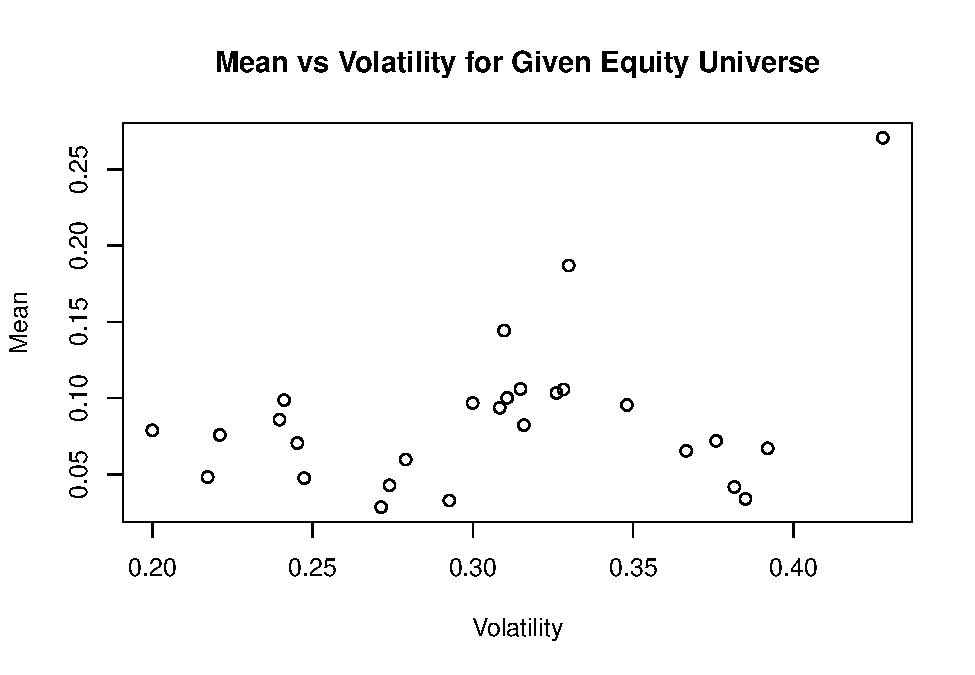
\includegraphics{hw3---siddharth-iyer_files/figure-latex/unnamed-chunk-4-1.pdf}

\begin{Shaded}
\begin{Highlighting}[]
\CommentTok{\# acf: both autocorrelation and autocovariance}

\FunctionTok{plot}\NormalTok{(acpr, }\AttributeTok{col=}\StringTok{"red"}\NormalTok{, }\AttributeTok{lag.max=}\DecValTok{20}\NormalTok{, }
     \AttributeTok{main=}\StringTok{"Autocorrelation of price changes"}\NormalTok{)}
\end{Highlighting}
\end{Shaded}

\includegraphics{hw3---siddharth-iyer_files/figure-latex/unnamed-chunk-4-2.pdf}

\begin{Shaded}
\begin{Highlighting}[]
\CommentTok{\# Roll estimate of bid{-}ask spread}

\NormalTok{covpr }\OtherTok{\textless{}{-}} \FunctionTok{acf}\NormalTok{(dpr, }\AttributeTok{lag.max=}\DecValTok{20}\NormalTok{, }\AttributeTok{type=}\StringTok{"covariance"}\NormalTok{, }\AttributeTok{plot=}\ConstantTok{FALSE}\NormalTok{)}

\NormalTok{gamma0 }\OtherTok{\textless{}{-}} \FunctionTok{sd}\NormalTok{(dpr)}\SpecialCharTok{\^{}}\DecValTok{2}
\CommentTok{\#print(gamma0)}

\NormalTok{gamma0alt }\OtherTok{\textless{}{-}}\NormalTok{ covpr}\SpecialCharTok{$}\NormalTok{acf[}\DecValTok{1}\NormalTok{]}
\CommentTok{\#print(gamma0alt)}

\NormalTok{gamma1 }\OtherTok{\textless{}{-}}\NormalTok{ covpr}\SpecialCharTok{$}\NormalTok{acf[}\DecValTok{2}\NormalTok{]}
\CommentTok{\#print(gamma1)}

\NormalTok{cparam}\FloatTok{.2} \OtherTok{\textless{}{-}} \FunctionTok{sqrt}\NormalTok{(}\SpecialCharTok{{-}}\NormalTok{covpr}\SpecialCharTok{$}\NormalTok{acf[}\DecValTok{2}\NormalTok{])}
\FunctionTok{cat}\NormalTok{(}\StringTok{"bid{-}ask spread (2*c): "}\NormalTok{, }\DecValTok{2}\SpecialCharTok{*}\NormalTok{cparam}\FloatTok{.2}\NormalTok{, }\StringTok{"}\SpecialCharTok{\textbackslash{}n}\StringTok{"}\NormalTok{)}
\end{Highlighting}
\end{Shaded}

\begin{verbatim}
## bid-ask spread (2*c):  0.0002112998
\end{verbatim}

\begin{Shaded}
\begin{Highlighting}[]
\NormalTok{sig2u }\OtherTok{\textless{}{-}}\NormalTok{ gamma0 }\SpecialCharTok{+} \DecValTok{2}\SpecialCharTok{*}\NormalTok{ gamma1}
\NormalTok{sigu}\FloatTok{.2} \OtherTok{\textless{}{-}} \FunctionTok{sqrt}\NormalTok{(sig2u)}
\FunctionTok{cat}\NormalTok{(}\StringTok{"sigma: "}\NormalTok{, sigu}\FloatTok{.2}\NormalTok{, }\StringTok{"}\SpecialCharTok{\textbackslash{}n}\StringTok{"}\NormalTok{)}
\end{Highlighting}
\end{Shaded}

\begin{verbatim}
## sigma:  0.0002380327
\end{verbatim}

When we are using log(price) and applying diff on the datasets, we are
effectively taking the spread on returns data. I don't this this makes
much sense.

Problem 3.1.3

\begin{Shaded}
\begin{Highlighting}[]
\NormalTok{realizedVar }\OtherTok{\textless{}{-}} \ControlFlowTok{function}\NormalTok{(q)\{}
\NormalTok{  pr }\OtherTok{\textless{}{-}} \FunctionTok{as.numeric}\NormalTok{(tqdata}\SpecialCharTok{$}\NormalTok{PRICE)}
  \FunctionTok{rCov}\NormalTok{(}\FunctionTok{diff}\NormalTok{(pr, }\AttributeTok{lag=}\NormalTok{q, }\AttributeTok{differences=}\DecValTok{1}\NormalTok{)}\SpecialCharTok{/}\NormalTok{q)}
\NormalTok{\}}
\CommentTok{\# compute the signature plot sigma.day(q) = sqrt(RV(q))}
\NormalTok{sig\_data }\OtherTok{\textless{}{-}} \ConstantTok{NULL}

\ControlFlowTok{for}\NormalTok{(q }\ControlFlowTok{in} \DecValTok{1}\SpecialCharTok{:}\DecValTok{100}\NormalTok{)\{}
\NormalTok{  sig\_data }\OtherTok{\textless{}{-}} \FunctionTok{c}\NormalTok{(sig\_data, }\FunctionTok{sqrt}\NormalTok{(}\FunctionTok{realizedVar}\NormalTok{(q)))}
\NormalTok{\}}

\FunctionTok{plot}\NormalTok{(sig\_data, }\AttributeTok{type =}\StringTok{"l"}\NormalTok{, }\AttributeTok{main=}\StringTok{"Signature plot"}\NormalTok{)}
\end{Highlighting}
\end{Shaded}

\includegraphics{hw3---siddharth-iyer_files/figure-latex/unnamed-chunk-5-1.pdf}

We can see that as the sampling interval decreases, the realizedVol goes
to 0 because it all cancels out. This makes sense because the volatility
is normally distributed around mean, so the with more data being
smoothed by the resample, the closer the realizedVol will be to 0.

This code is taken from the lectures.

Problem 3.1.4

\begin{Shaded}
\begin{Highlighting}[]
\NormalTok{n\_trades }\OtherTok{=} \FunctionTok{length}\NormalTok{(tqdata)}
\NormalTok{q\_5min }\OtherTok{=}\NormalTok{ n\_trades}\SpecialCharTok{*}\DecValTok{5}\SpecialCharTok{/}\DecValTok{390}
\FunctionTok{cat}\NormalTok{(}\StringTok{"Realized Var: "}\NormalTok{, q\_5min}\SpecialCharTok{*}\FunctionTok{realizedVar}\NormalTok{(q\_5min), }\StringTok{"}\SpecialCharTok{\textbackslash{}n}\StringTok{"}\NormalTok{)}
\end{Highlighting}
\end{Shaded}

\begin{verbatim}
## Realized Var:  12.79712
\end{verbatim}

\begin{Shaded}
\begin{Highlighting}[]
\NormalTok{sig\_roll }\OtherTok{=} \FunctionTok{sqrt}\NormalTok{(n\_trades }\SpecialCharTok{*}\NormalTok{ (sigu}\FloatTok{.1}\NormalTok{)}\SpecialCharTok{\^{}}\DecValTok{2}\NormalTok{)}
\FunctionTok{cat}\NormalTok{(}\StringTok{"Roll: "}\NormalTok{, sig\_roll, }\StringTok{"}\SpecialCharTok{\textbackslash{}n}\StringTok{"}\NormalTok{)}
\end{Highlighting}
\end{Shaded}

\begin{verbatim}
## Roll:  12.32414
\end{verbatim}

Incredible! The Roll model and the Realized volatility is approximately
the same at a log of 5 minutes.

\end{document}
